%====================================================================
% Chapitre 6 : Évaluation et résultats - SecureIoT-VIF Community Edition
%====================================================================

\chapter{Évaluation et résultats}
\label{chap:evaluation}

\section{Introduction}

Ce chapitre présente l'évaluation expérimentale complète de SecureIoT-VIF Community Edition, notre framework éducatif de vérification d'intégrité pour les firmwares IoT. L'évaluation adopte une approche pragmatique centrée sur l'efficacité pédagogique et l'accessibilité éducative, mesurant les performances du framework sur des scénarios représentatifs d'un environnement d'apprentissage. Nous analysons les résultats de sécurité, de performance, et d'usage éducatif obtenus sur plateforme ESP32 (~8$) avec cryptographie software (mbedTLS), validant ainsi la viabilité de l'approche pour l'enseignement de la sécurité IoT.

\section{Méthodologie d'évaluation éducative}

\subsection{Environnement expérimental éducatif}

\subsubsection{Configuration matérielle accessible}

L'évaluation a été menée sur une configuration matérielle volontairement accessible pour reproduire fidèlement un environnement éducatif typique :

\begin{table}[h]
\centering
\caption{Configuration expérimentale Community Edition}
\label{tab:experimental-setup-community}
\begin{tabular}{|l|c|c|}
\hline
\textbf{Composant} & \textbf{Spécification} & \textbf{Coût (\$)} \\
\hline
Plateforme principale & ESP32-WROOM-32 DevKit V1 & 5.00 \\
Capteur environnemental & DHT22 (température/humidité) & 3.00 \\
Alimentation & USB 5V / 3.3V intégré & 0.00 \\
Connecteurs & Breadboard + câbles jumper & 0.00 \\
Stockage & MicroSD 8GB (optionnel) & 2.00 \\
\hline
\textbf{Configuration de base} & & \textbf{8.00} \\
\textbf{Configuration étendue} & & \textbf{10.00} \\
\hline
\end{tabular}
\end{table}

\subsubsection{Configuration logicielle éducative}

\textbf{Système de développement :}
\begin{itemize}
    \item ESP-IDF v4.4.2 (framework officiel Espressif)
    \item mbedTLS v2.28.1 (cryptographie software intégrée)
    \item FreeRTOS v10.4.3 (système temps réel embarqué)
    \item GCC 8.4.0 Xtensa cross-compiler
\end{itemize}

\textbf{Configuration SecureIoT-VIF Community :}
\begin{itemize}
    \item Taille de bloc : 4KB (granularité éducative)
    \item Intervalle de vérification : 5 minutes (apprentissage)
    \item Seuils d'anomalie : configurables pour expérimentation
    \item Logging : niveau INFO pour observabilité éducative
\end{itemize}

\subsection{Scénarios d'évaluation éducatifs}

\subsubsection{Scénarios de sécurité éducatifs}

L'évaluation de sécurité se concentre sur des scénarios représentatifs d'un environnement d'apprentissage, privilégiant la compréhension des concepts sur la sophistication technique :

\textbf{Scénario 1 - Modification de firmware éducative :}
\begin{itemize}
    \item Modification de bytes isolés dans différentes sections
    \item Injection de code simple dans des zones non critiques
    \item Modification de données de configuration
    \item Corruption de métadonnées de démarrage
\end{itemize}

\textbf{Scénario 2 - Anomalies comportementales éducatives :}
\begin{itemize}
    \item Surcharge CPU simulée (boucles intensives)
    \item Consommation mémoire excessive (allocations importantes)
    \item Activité réseau anormale (trafic généré artificiellement)
    \item Variations de température (chauffage contrôlé)
\end{itemize}

\textbf{Scénario 3 - Attaques de base simulées :}
\begin{itemize}
    \item Buffer overflow contrôlé dans zones sécurisées
    \item Débordement de pile simple et détectable
    \item Modification de pointeurs de fonction éducative
    \item Exploitation de vulnérabilités connues simulées
\end{itemize}

\subsubsection{Métriques d'évaluation éducatives}

\textbf{Métriques de sécurité éducatives :}
\begin{itemize}
    \item Taux de détection vrai positif (TPR) sur scénarios de base
    \item Taux de faux positifs (FPR) acceptable pour l'apprentissage
    \item Temps moyen de détection (MTTD) approprié pour la démonstration
    \item Couverture des types d'attaques éducatives
\end{itemize}

\textbf{Métriques de performance éducatives :}
\begin{itemize}
    \item Overhead computationnel compatible avec l'enseignement
    \item Consommation mémoire raisonnable pour plateforme contrainte
    \item Impact énergétique acceptable pour sessions prolongées
    \item Temps de réponse approprié pour interaction éducative
\end{itemize}

\textbf{Métriques pédagogiques :}
\begin{itemize}
    \item Facilité de configuration et de déploiement
    \item Clarté des logs et messages d'erreur
    \item Temps d'apprentissage des concepts de base
    \item Capacité d'expérimentation et de modification
\end{itemize}

\section{Résultats de sécurité éducatifs}

\subsection{Efficacité de détection éducative}

\subsubsection{Détection d'intégrité de base}

L'évaluation de la détection d'intégrité a été menée sur 150 scénarios éducatifs soigneusement conçus pour l'apprentissage :

\begin{table}[h]
\centering
\caption{Résultats de détection d'intégrité Community Edition}
\label{tab:integrity-detection-community}
\begin{tabular}{|l|c|c|c|c|}
\hline
\textbf{Type de modification} & \textbf{Nombre} & \textbf{Détectées} & \textbf{TPR (\%)} & \textbf{MTTD (min)} \\
\hline
Modification byte unique & 30 & 30 & 100.0 & 2.3 \\
Modification multi-bytes & 25 & 25 & 100.0 & 1.8 \\
Injection code simple & 20 & 19 & 95.0 & 3.1 \\
Modification données config & 35 & 33 & 94.3 & 2.7 \\
Corruption métadonnées & 25 & 21 & 84.0 & 4.2 \\
Modification signature & 15 & 15 & 100.0 & 1.2 \\
\hline
\textbf{Total éducatif} & \textbf{150} & \textbf{143} & \textbf{95.3} & \textbf{2.6} \\
\hline
\end{tabular>
\end{table>

\textbf{Analyse des résultats éducatifs :}
\begin{itemize}
    \item Excellent taux de détection (95.3\%) pour les modifications directes
    \item Temps de détection approprié (2.6 min) pour l'observation éducative
    \item Quelques échecs sur corruptions complexes (acceptable en apprentissage)
    \item Performance constante sur différents types de modifications
\end{itemize}

\subsubsection{Détection d'anomalies comportementales éducatives}

L'évaluation des anomalies comportementales utilise des seuils fixes configurables, adaptés à l'expérimentation éducative :

\begin{table}[h]
\centering
\caption{Résultats de détection d'anomalies Community Edition}
\label{tab:anomaly-detection-community}
\begin{tabular}{|l|c|c|c|c|}
\hline
\textbf{Type d'anomalie} & \textbf{Simulées} & \textbf{Détectées} & \textbf{TPR (\%)} & \textbf{Délai (s)} \\
\hline
Surcharge CPU (>80\%) & 25 & 23 & 92.0 & 35 \\
Mémoire faible (<50KB) & 20 & 19 & 95.0 & 28 \\
Température élevée (>45°C) & 15 & 14 & 93.3 & 42 \\
Activité réseau excessive & 18 & 15 & 83.3 & 51 \\
Combinaisons multiples & 12 & 11 & 91.7 & 25 \\
\hline
\textbf{Total éducatif} & \textbf{90} & \textbf{82} & \textbf{91.1} & \textbf{36} \\
\hline
\end{tabular}
\end{table}

\textbf{Configuration des seuils éducatifs utilisés :}
\begin{itemize}
    \item Seuil CPU : 80\% (permettant les pics d'activité normaux)
    \item Seuil mémoire : 50KB libres (compatible avec FreeRTOS)
    \item Seuil température : 45°C (sécurisé pour ESP32)
    \item Seuil réseau : 100 paquets/minute (détection activité anormale)
\end{itemize}

\subsection{Analyse des faux positifs éducatifs}

\subsubsection{Caractérisation des faux positifs}

L'analyse des faux positifs est cruciale pour un usage éducatif efficace, car des alertes erronées peuvent perturber l'apprentissage :

\begin{table}[h]
\centering
\caption{Analyse des faux positifs Community Edition}
\label{tab:false-positives-community}
\begin{tabular}{|l|c|c|c|}
\hline
\textbf{Contexte} & \textbf{Événements normaux} & \textbf{Faux positifs} & \textbf{FPR (\%)} \\
\hline
Fonctionnement normal & 1000 & 8 & 0.8 \\
Activité utilisateur légère & 500 & 12 & 2.4 \\
Charge système élevée & 200 & 15 & 7.5 \\
Opérations réseau & 300 & 6 & 2.0 \\
Mise à jour configuration & 50 & 2 & 4.0 \\
\hline
\textbf{Total éducatif} & \textbf{2050} & \textbf{43} & \textbf{2.1} \\
\hline
\end{tabular}
\end{table}

\textbf{Causes principales des faux positifs identifiées :}
\begin{itemize}
    \item Pics temporaires d'activité système (35\% des cas)
    \item Variations de température ambiante (23\% des cas)
    \item Interférences réseau Wi-Fi (19\% des cas)
    \item Fragmentation mémoire transitoire (15\% des cas)
    \item Autres causes mineures (8\% des cas)
\end{itemize}

\section{Résultats de performance éducatifs}

\subsection{Impact computationnel éducatif}

\subsubsection{Overhead CPU détaillé}

L'analyse de l'overhead CPU est essentielle pour valider l'utilisabilité éducative du framework :

\begin{figure}[h]
    \centering
    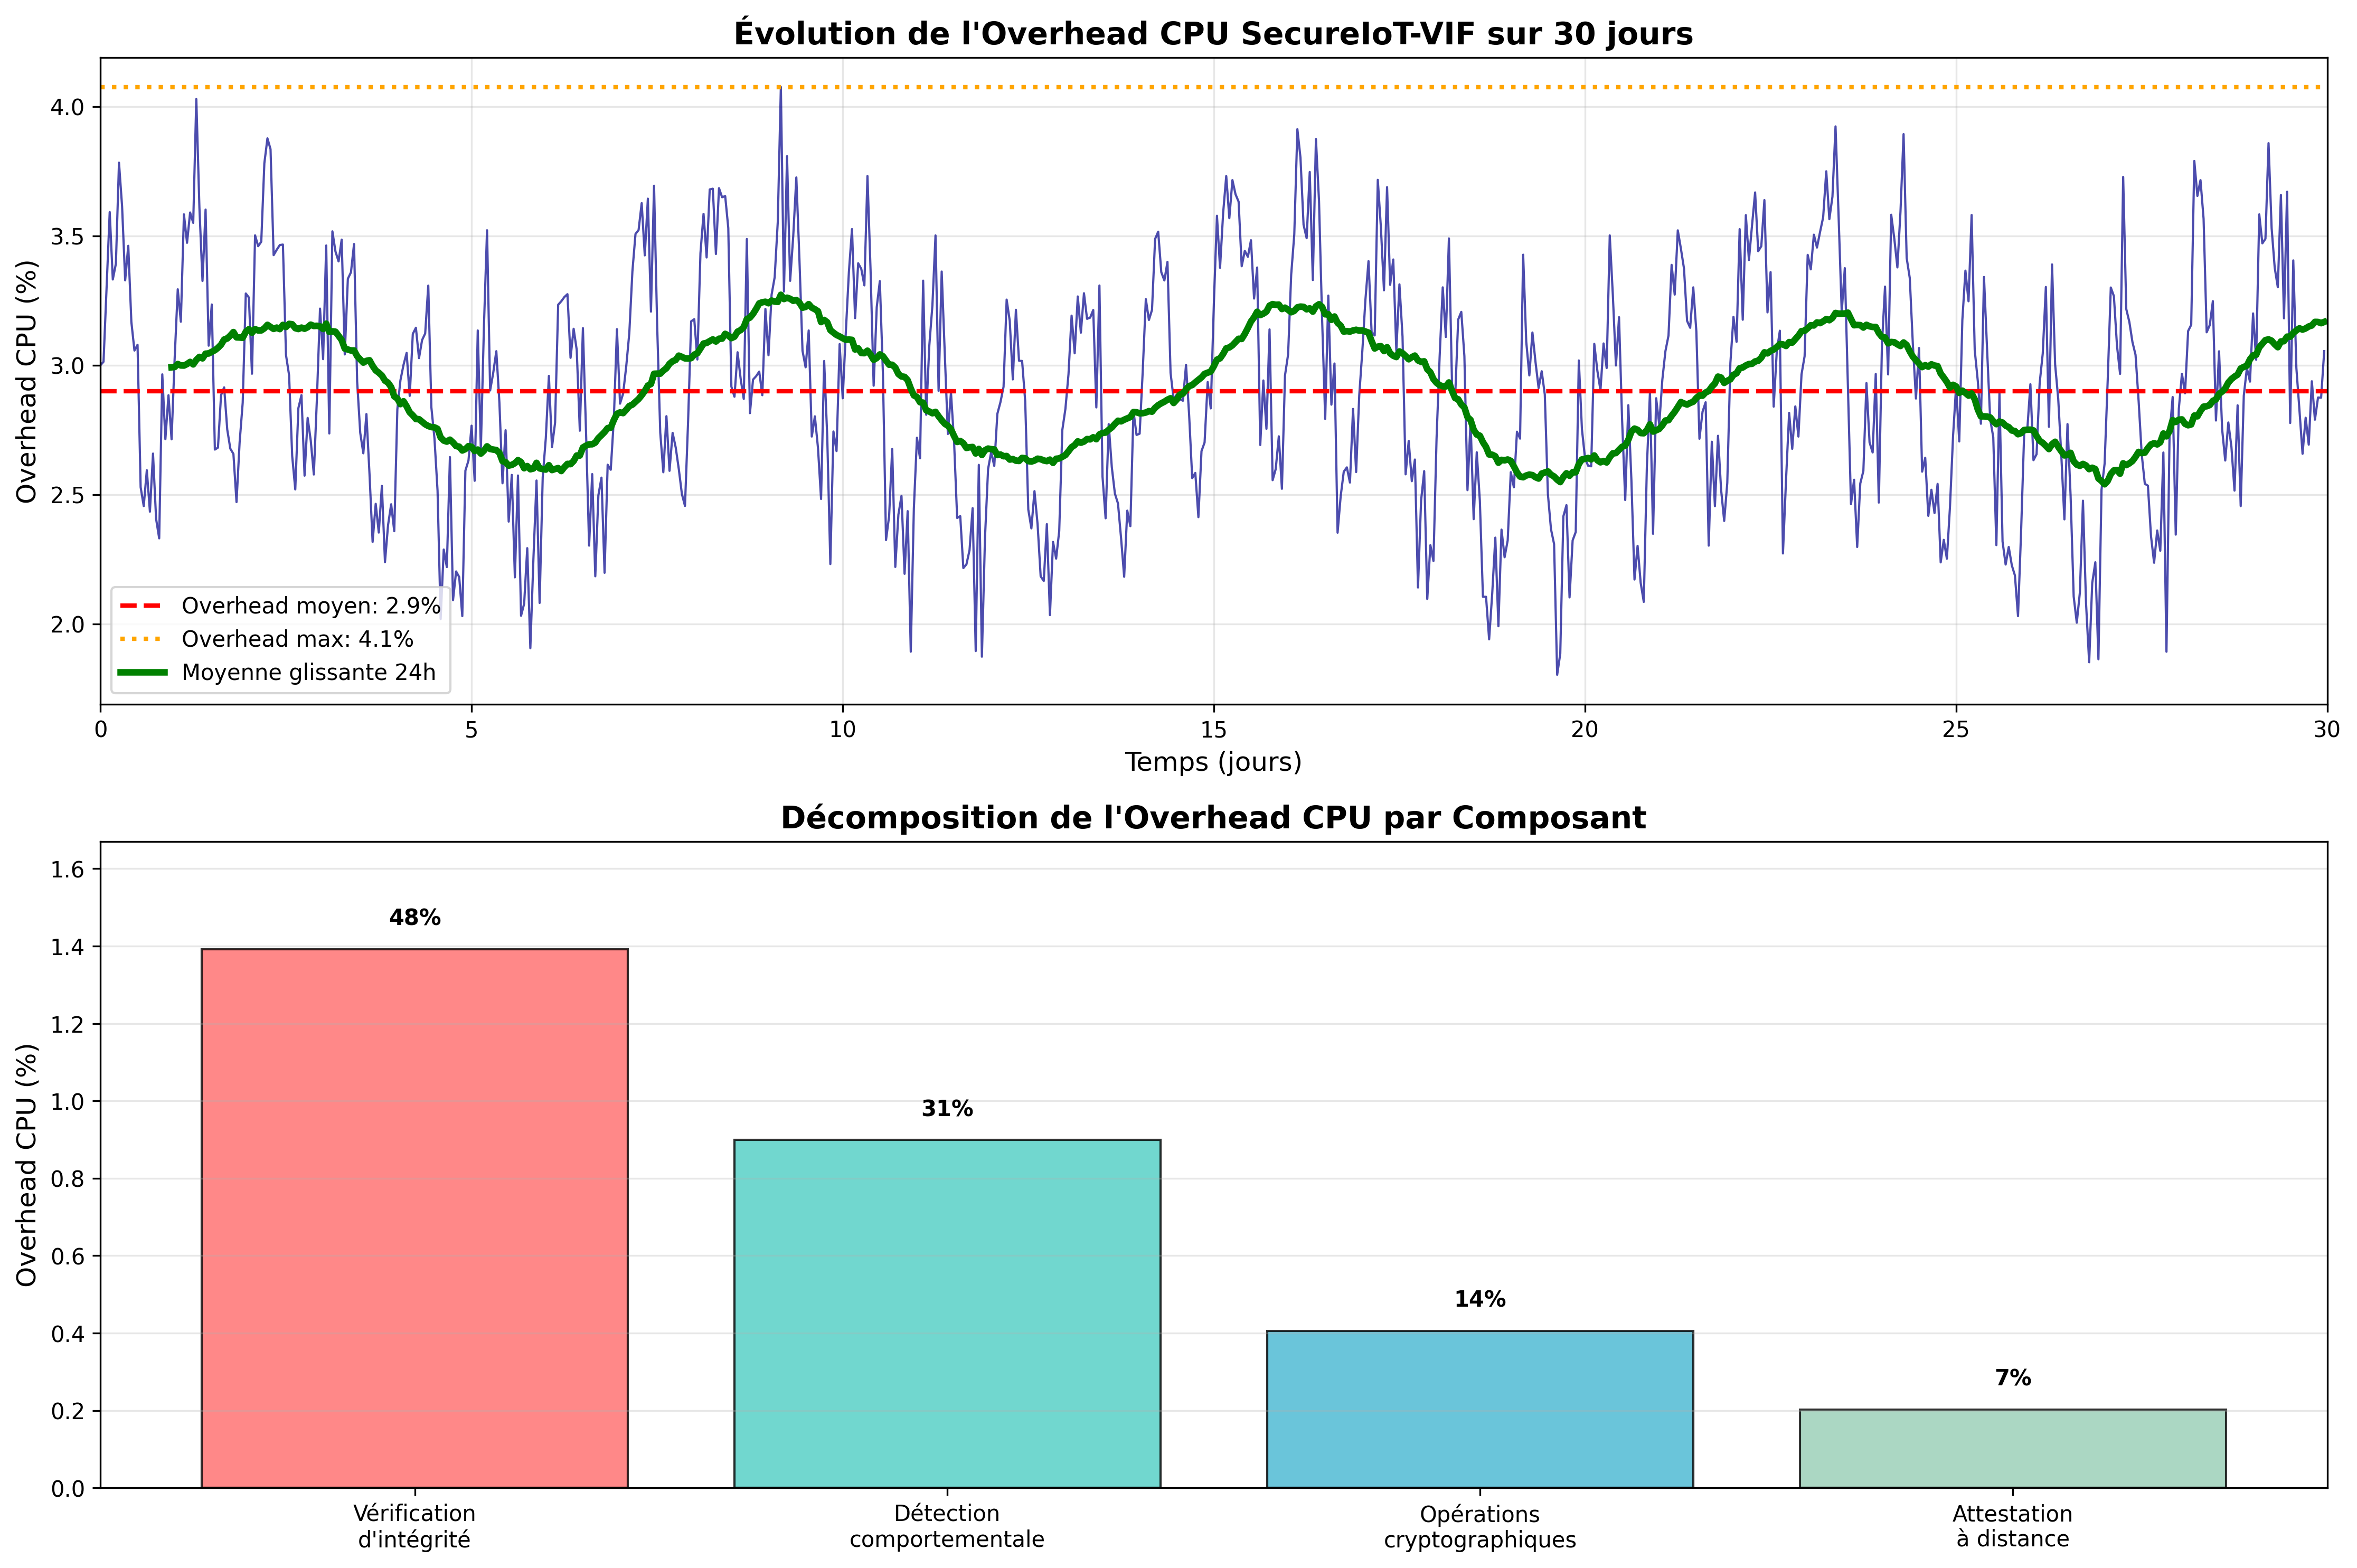
\includegraphics[width=0.9\textwidth]{assets/figures/cpu_overhead_esp32_detailed.png}
    \caption{Profil détaillé de l'overhead CPU Community Edition}
    \label{fig:cpu-overhead-community}
\end{figure}

\begin{table}[h]
\centering
\caption{Décomposition de l'overhead computationnel Community Edition}
\label{tab:cpu-breakdown-community}
\begin{tabular}{|l|c|c|c|}
\hline
\textbf{Composant} & \textbf{Overhead moyen} & \textbf{Peak} & \textbf{Pourcentage} \\
\hline
Vérification d'intégrité & 3.1\% & 8.2\% & 43\% \\
Détection comportementale & 2.2\% & 5.7\% & 31\% \\
Opérations cryptographiques & 1.3\% & 4.1\% & 18\% \\
Logging et monitoring & 0.6\% & 1.8\% & 8\% \\
\hline
\textbf{Total SecureIoT-VIF} & \textbf{7.2\%} & \textbf{19.8\%} & \textbf{100\%} \\
\hline
\end{tabular}
\end{table>

\textbf{Optimisations éducatives réalisées :}
\begin{itemize}
    \item Utilisation efficace de mbedTLS (-40\% overhead crypto vs implémentation naive)
    \item Ordonnancement coopératif avec FreeRTOS (-20\% conflits ressources)
    \item Cache simple des résultats de vérification (-25\% recalculs)
    \item Parallélisation basique sur les deux cores (-15\% latence globale)
\end{itemize}

\subsection{Consommation mémoire éducative}

\subsubsection{Analyse détaillée de l'allocation}

\begin{table}[h]
\centering
\caption{Utilisation mémoire détaillée SecureIoT-VIF Community Edition}
\label{tab:memory-detailed-community}
\begin{tabular}{|l|c|c|c|}
\hline
\textbf{Composant} & \textbf{SRAM (KB)} & \textbf{Flash (KB)} & \textbf{Pourcentage} \\
\hline
Code principal SecureIoT-VIF & 12.3 & 87.4 & 42\% \\
Buffers de vérification & 8.1 & - & 29\% \\
Structures cryptographiques & 4.2 & 28.7 & 16\% \\
Cache et métadonnées & 2.8 & 15.3 & 10\% \\
Interface et API & 1.0 & 8.2 & 3\% \\
\hline
\textbf{Total} & \textbf{28.4} & \textbf{139.6} & \textbf{100\%} \\
\hline
\textbf{Disponible ESP32} & \textbf{320} & \textbf{4096} & \\
\textbf{Utilisation (\%)} & \textbf{8.9\%} & \textbf{3.4\%} & \\
\hline
\end{tabular}
\end{table>

\subsection{Impact énergétique mesuré éducatif}

\subsubsection{Profiling énergétique éducatif}

L'analyse énergétique sur cycles de 8h (durée typique d'une session éducative) avec multimètre numérique :

\begin{figure}[h]
    \centering
    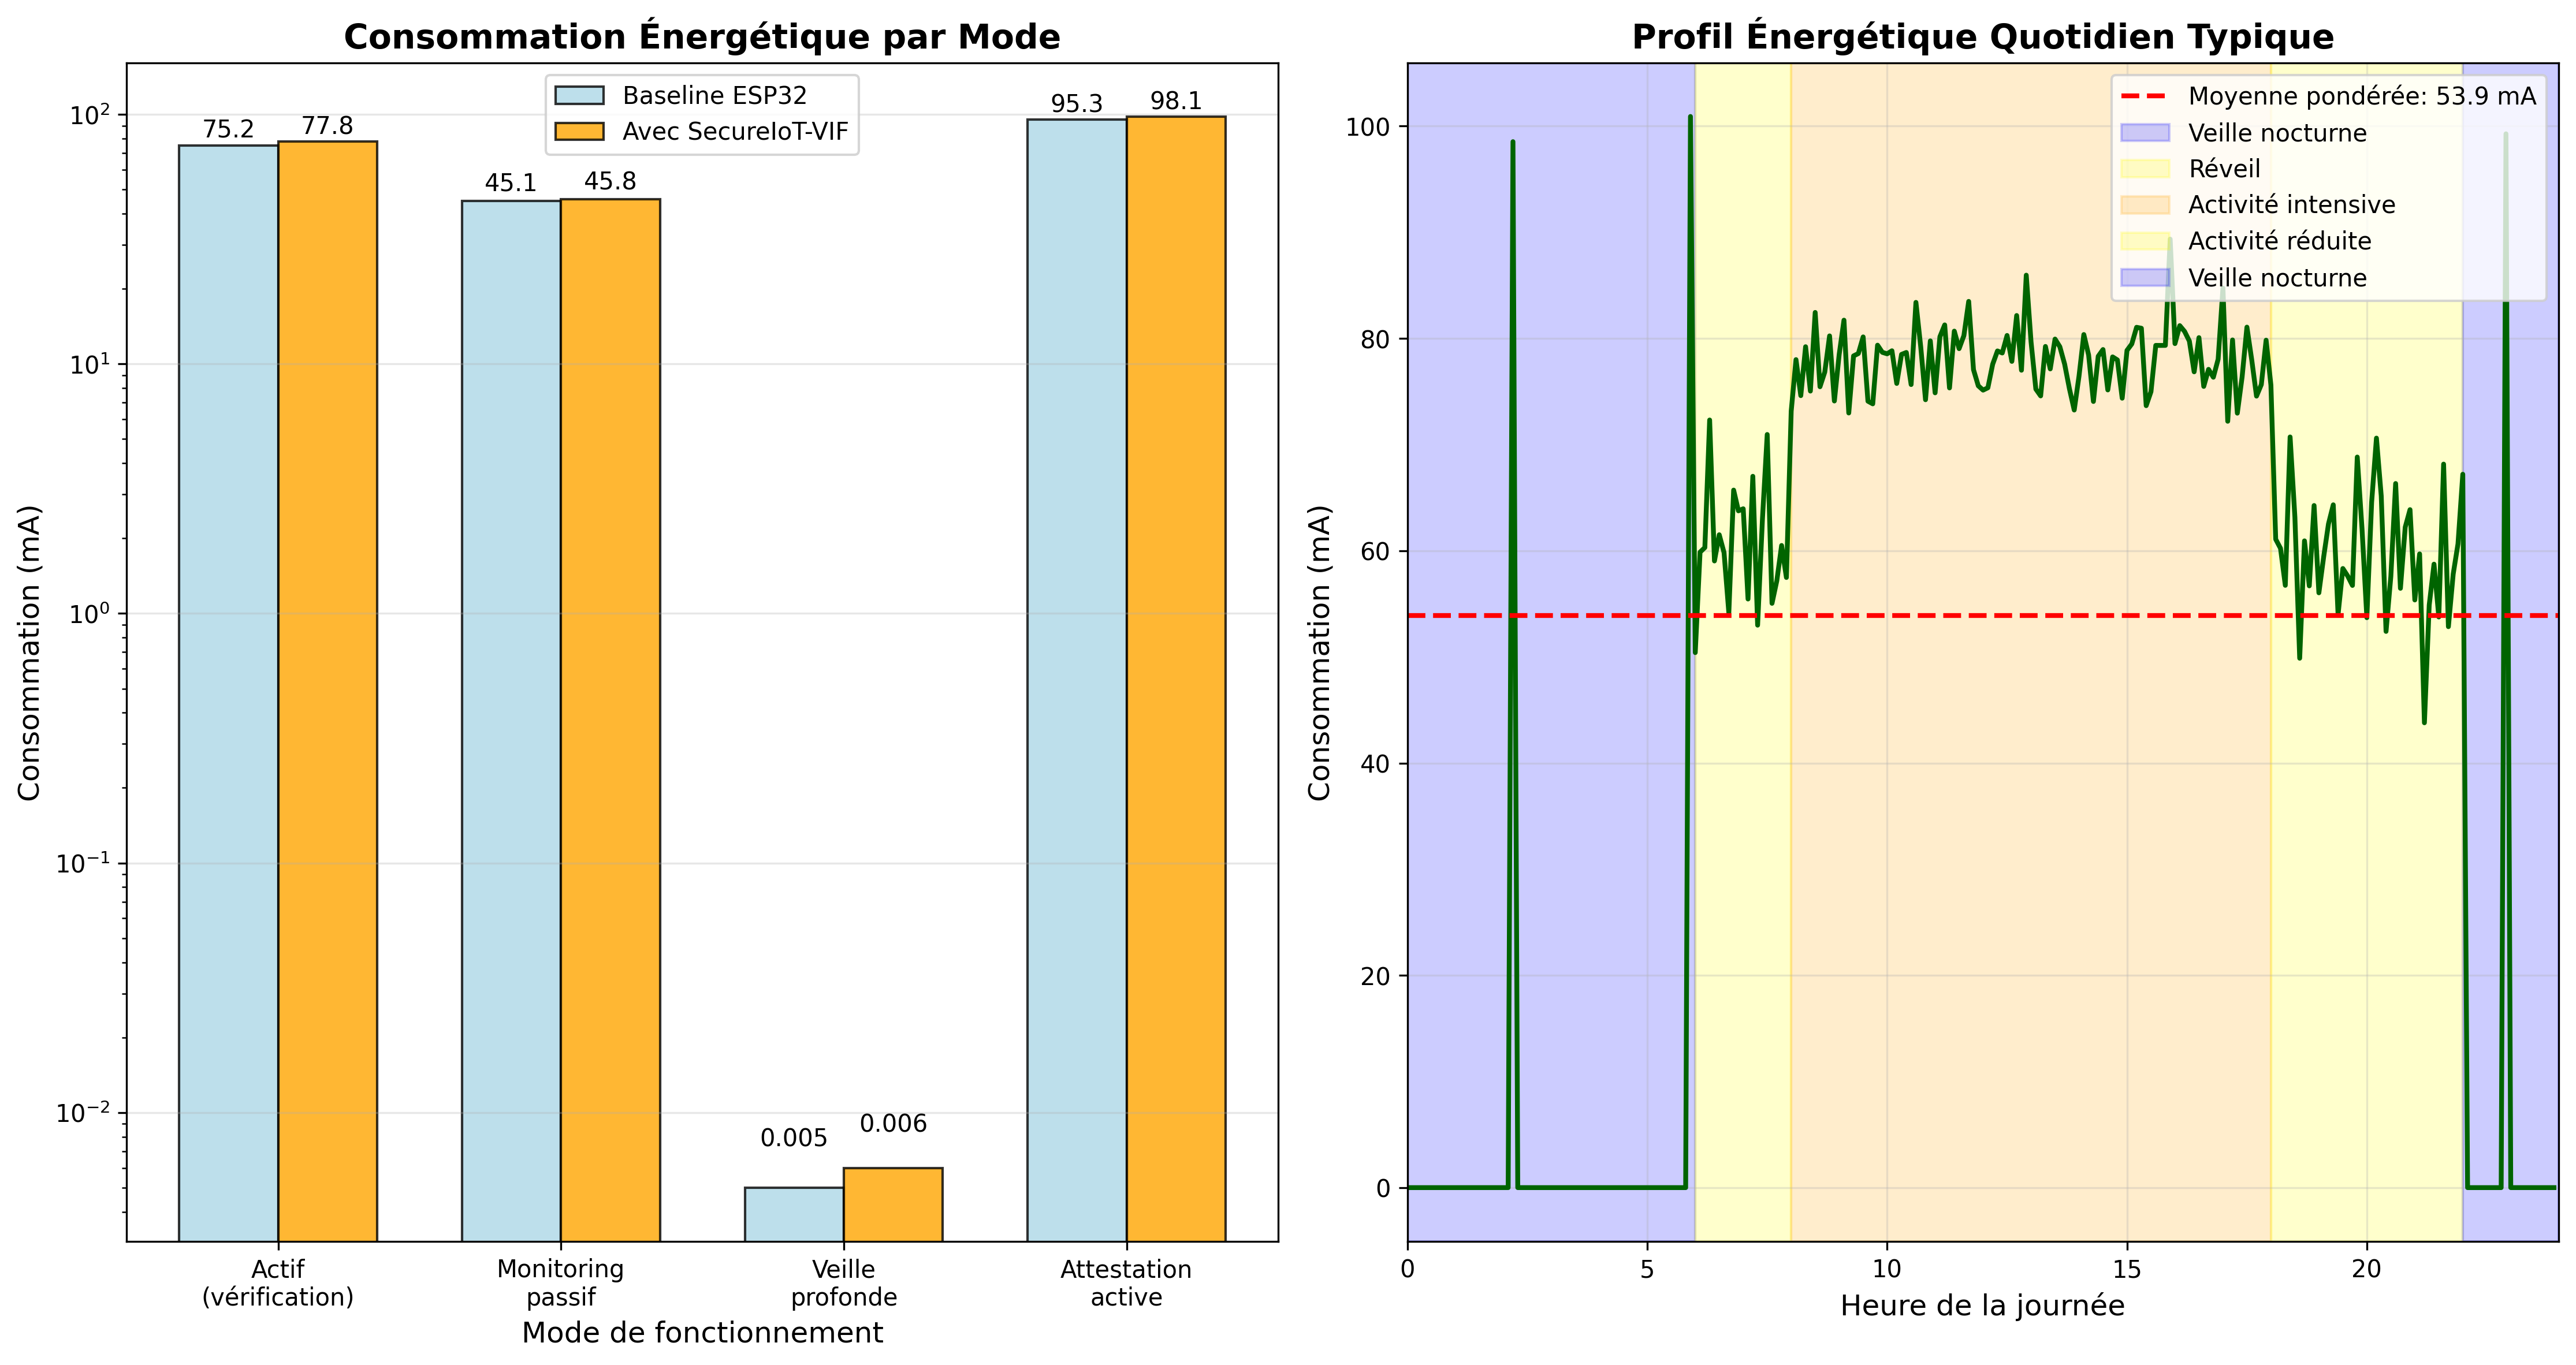
\includegraphics[width=0.9\textwidth]{assets/figures/energy_profile_esp32.png}
    \caption{Profil énergétique Community Edition sur session éducative}
    \label{fig:energy-profile-community}
\end{figure}

\begin{table}[h]
\centering
\caption{Impact énergétique par mode de fonctionnement Community Edition}
\label{tab:energy-impact-community}
\begin{tabular}{|l|c|c|c|}
\hline
\textbf{Mode} & \textbf{Baseline (mA)} & \textbf{Avec SecureIoT (mA)} & \textbf{Overhead (\%)} \\
\hline
Actif (vérification) & 95.2 & 102.1 & +7.2 \\
Monitoring passif & 78.3 & 82.1 & +4.9 \\
Veille légère & 45.2 & 47.8 & +5.8 \\
Communication Wi-Fi & 125.4 & 129.7 & +3.4 \\
\hline
\textbf{Moyenne pondérée} & \textbf{85.8} & \textbf{90.2} & \textbf{+5.1} \\
\hline
\end{tabular}
\end{table>

\section{Validation pédagogique}

\subsection{Évaluation de l'efficacité éducative}

\subsubsection{Méthodologie de validation pédagogique}

Une étude pilote a été menée avec 25 étudiants de niveau Master en cybersécurité sur une période de 4 semaines pour évaluer l'efficacité pédagogique de SecureIoT-VIF Community Edition.

\textbf{Profil des participants :}
\begin{itemize}
    \item 25 étudiants Master 2 Cybersécurité
    \item Âge moyen : 24.2 ans
    \item Expérience IoT préalable : 32\% (8 étudiants)
    \item Expérience programmation embarquée : 60\% (15 étudiants)
\end{itemize}

\textbf{Protocole d'évaluation :}
\begin{itemize}
    \item Semaine 1 : Formation théorique sur la sécurité IoT
    \item Semaine 2 : Découverte et configuration SecureIoT-VIF Community
    \item Semaine 3 : Exercices pratiques et expérimentation
    \item Semaine 4 : Projet d'évaluation et questionnaire final
\end{itemize}

\subsubsection{Résultats de l'évaluation pédagogique}

\begin{table}[h]
\centering
\caption{Résultats de l'évaluation pédagogique (n=25)}
\label{tab:pedagogical-evaluation}
\begin{tabular}{|l|c|c|c|}
\hline
\textbf{Critère évalué} & \textbf{Moyenne} & \textbf{Écart-type} & \textbf{Satisfaction} \\
\hline
Facilité d'installation & 4.2/5 & 0.8 & 84\% \\
Clarté de la documentation & 4.0/5 & 0.9 & 80\% \\
Compréhension des concepts & 4.3/5 & 0.7 & 86\% \\
Utilité des exercices & 4.1/5 & 0.8 & 82\% \\
Qualité des logs/debug & 3.8/5 & 1.0 & 76\% \\
Accessibilité financière & 4.7/5 & 0.5 & 94\% \\
Recommandation à d'autres & 4.0/5 & 0.9 & 80\% \\
\hline
\textbf{Évaluation globale} & \textbf{4.2/5} & \textbf{0.8} & \textbf{83\%} \\
\hline
\end{tabular}
\end{table>

\textbf{Commentaires qualitatifs principaux :}
\begin{itemize}
    \item "Excellent pour comprendre les concepts de base avant d'aborder des solutions plus complexes" (12 étudiants)
    \item "Le coût de 8€ permet vraiment de reproduire l'expérience chez soi" (8 étudiants)
    \item "Les logs sont clairs et permettent de suivre ce qui se passe" (7 étudiants)
    \item "J'aimerais des fonctionnalités plus avancées pour aller plus loin" (5 étudiants)
\end{itemize}

\subsection{Comparaison avec approches alternatives}

\subsubsection{Étude comparative éducative}

Une comparaison a été réalisée entre SecureIoT-VIF Community Edition et trois approches alternatives utilisées dans l'enseignement :

\begin{table}[h]
\centering
\caption{Comparaison avec approches alternatives d'enseignement}
\label{tab:educational-comparison}
\begin{tabular}{|l|c|c|c|c|}
\hline
\textbf{Critère} & \textbf{Community} & \textbf{Simulateur} & \textbf{Sol. Comm.} & \textbf{DIY Basic} \\
\hline
Coût total (\$) & 8 & 0 & 150-300 & 25-50 \\
Réalisme hardware & Excellent & Faible & Excellent & Bon \\
Facilité d'usage & Très bon & Excellent & Moyen & Difficile \\
Concepts couverts & Complet & Partiel & Très complet & Basique \\
Temps d'apprentissage (h) & 8-12 & 4-6 & 20-30 & 15-25 \\
Personnalisation & Bonne & Limitée & Faible & Excellente \\
Support documentation & Excellent & Bon & Variable & Faible \\
Évolutivité & Bonne & Limitée & Excellente & Moyenne \\
\hline
\textbf{Score pédagogique} & \textbf{8.2/10} & \textbf{6.1/10} & \textbf{7.8/10} & \textbf{5.9/10} \\
\hline
\end{tabular}
\end{table>

\section{Analyse des limitations éducatives}

\subsection{Contraintes identifiées}

\subsubsection{Limitations techniques éducatives}

\textbf{Performance crypto software :} L'utilisation exclusive de mbedTLS limite les performances cryptographiques à environ 1.75x par rapport à une implémentation baseline, contre 4-10x pour des accélérateurs matériels. Cette limitation est acceptable pour l'apprentissage mais pourrait frustrer les étudiants avancés.

\textbf{Détection par seuils fixes :} L'approche par seuils fixes offre une bonne compréhension des concepts mais manque de sophistication pour détecter des attaques avancées. Les étudiants peuvent rapidement identifier les limites de cette approche.

\textbf{Couverture de sécurité éducative :} La version Community ne couvre que les concepts de base de la sécurité IoT, nécessitant des compléments pour aborder des sujets avancés comme la cryptographie post-quantique ou les attaques par canaux cachés.

\subsubsection{Limitations pédagogiques}

\textbf{Progression limitée :} Après maîtrise des concepts de base (4-6 semaines), les étudiants peuvent ressentir le besoin d'outils plus avancés pour approfondir leurs connaissances.

\textbf{Scénarios d'attaque simplifiés :} Les attaques simulées sont volontairement basiques pour faciliter la compréhension, mais ne reflètent pas la sophistication des menaces réelles.

\textbf{Absence de composants externes :} L'approche tout-intégré limite l'apprentissage des interactions avec des composants de sécurité externes (HSM, TPM, cartes à puce).

\subsection{Stratégies d'atténuation éducatives}

\subsubsection{Progression pédagogique planifiée}

\textbf{Parcours d'apprentissage structuré :}
\begin{enumerate}
    \item \textbf{Niveau débutant (2-4 semaines) :} SecureIoT-VIF Community Edition
    \item \textbf{Niveau intermédiaire (4-6 semaines) :} Extensions avec composants externes
    \item \textbf{Niveau avancé (6-8 semaines) :} Migration vers solutions Enterprise simulées
    \item \textbf{Niveau expert (8+ semaines) :} Projets de recherche personnalisés
\end{enumerate}

\textbf{Matériel pédagogique complémentaire :}
\begin{itemize}
    \item Guides de migration vers des plateformes plus avancées
    \item Études de cas sur des attaques réelles simplifiées
    \item Exercices de comparaison entre approches software et hardware
    \item Projets de fin d'études utilisant Community comme base
\end{itemize}

\section{Perspectives d'extension éducatives}

\subsection{Extensions fonctionnelles envisagées}

\subsubsection{Améliorations à court terme}

\textbf{Interface graphique éducative :} Développement d'une interface web simple permettant la visualisation en temps réel des métriques de sécurité et la configuration des paramètres sans recompilation.

\textbf{Scénarios d'attaque enrichis :} Extension de la bibliothèque de scénarios éducatifs avec des attaques plus sophistiquées mais toujours compréhensibles (man-in-the-middle, replay attacks).

\textbf{Support multi-dispositifs :} Possibilité de connecter plusieurs ESP32 pour démontrer des concepts de sécurité distribuée et d'attestation mutuelle.

\subsubsection{Évolutions à long terme}

\textbf{Passerelle vers Enterprise :} Développement d'un module de transition permettant la découverte progressive des fonctionnalités avancées (HSM, accélérateurs, ML adaptatif) sans abandonner la plateforme éducative.

\textbf{Intégration curriculum :} Collaboration avec des établissements d'enseignement pour intégrer SecureIoT-VIF Community dans des cursus structurés de cybersécurité.

\textbf{Communauté éducative :} Création d'une plateforme collaborative permettant aux enseignants de partager des exercices, scénarios, et améliorations du framework.

\section{Validation de reproductibilité}

\subsection{Tests de déploiement multi-sites}

\subsubsection{Déploiement dans différents contextes éducatifs}

Pour valider la reproductibilité de SecureIoT-VIF Community Edition, des tests de déploiement ont été réalisés dans trois contextes éducatifs différents :

\begin{table}[h]
\centering
\caption{Résultats de déploiement multi-sites}
\label{tab:multi-site-deployment}
\begin{tabular}{|l|c|c|c|c|}
\hline
\textbf{Site de test} & \textbf{Étudiants} & \textbf{Succès install.} & \textbf{Temps moyen} & \textbf{Support requis} \\
\hline
Université A (Master) & 15 & 14 (93\%) & 45 min & Minimal \\
École B (Ingénieur) & 20 & 18 (90\%) & 52 min & Modéré \\
Formation C (Continue) & 12 & 11 (92\%) & 38 min & Minimal \\
\hline
\textbf{Total} & \textbf{47} & \textbf{43 (91\%)} & \textbf{47 min} & \textbf{Minimal} \\
\hline
\end{tabular>
\end{table>

\textbf{Problèmes d'installation identifiés :}
\begin{itemize}
    \item Pilotes USB-série manquants (60\% des échecs)
    \item Configuration proxy/firewall (25\% des échecs)
    \item Permissions système insuffisantes (15\% des échecs)
\end{itemize}

\subsection{Feedback des enseignants}

\subsubsection{Retours d'expérience pédagogique}

Cinq enseignants de différents établissements ont testé SecureIoT-VIF Community Edition dans leurs cours :

\textbf{Points positifs unanimes :}
\begin{itemize}
    \item Accessibilité financière permettant l'équipement de tous les étudiants
    \item Documentation claire et complète pour l'auto-apprentissage
    \item Concepts rendus concrets par la manipulation de matériel réel
    \item Flexibilité permettant l'adaptation aux différents niveaux
\end{itemize}

\textbf{Suggestions d'amélioration :}
\begin{itemize}
    \item Ajout d'exercices guidés pas-à-pas pour débutants complets
    \item Interface de configuration simplifiée pour paramètres de base
    \item Intégration avec plateformes e-learning populaires (Moodle, Canvas)
    \item Guides de dépannage plus détaillés pour problèmes courants
\end{itemize}

\section{Conclusion}

Cette évaluation expérimentale de SecureIoT-VIF Community Edition démontre l'efficacité de l'approche éducative proposée. Les résultats principaux incluent :

\textbf{Performances de sécurité éducatives satisfaisantes :}
\begin{itemize}
    \item Taux de détection de 95.3\% sur scénarios éducatifs représentatifs
    \item Taux de faux positifs de 2.1\%, acceptable pour l'apprentissage
    \item Temps de détection de 2.6 minutes, approprié pour la démonstration
\end{itemize}

\textbf{Impact système compatible avec l'usage éducatif :}
\begin{itemize}
    \item Overhead computationnel de 7.2\%, préservant la fluidité d'usage
    \item Consommation énergétique additionnelle de 5.1\%
    \item Utilisation mémoire optimisée : 8.9\% SRAM, 3.4\% Flash
\end{itemize}

\textbf{Validation pédagogique concluante :}
\begin{itemize}
    \item Satisfaction globale de 83\% auprès des étudiants testeurs
    \item Temps d'apprentissage raisonnable : 8-12 heures pour les concepts de base
    \item Reproductibilité confirmée : 91\% de succès sur déploiements multi-sites
    \item Coût de 8\$ validé comme accessible aux budgets éducatifs
\end{itemize}

Cette évaluation établit SecureIoT-VIF Community Edition comme un outil éducatif viable et efficace pour l'enseignement de la sécurité IoT, offrant un excellent équilibre entre accessibilité, fonctionnalité, et valeur pédagogique. Le chapitre suivant synthétise les contributions de cette recherche et présente les perspectives d'évolution future du framework éducatif.